\chapter{基本的な使い方}
\section{PDF ファイル作成方法}
このへたれテンプレートには Makefile が付属するので
\begin{verbatim}
% make
\end{verbatim}
で PDF ファイルを作成できます.
\section{コメントアウト}
\% 以降はコメントアウトされます.
% 以降はコメントアウトされます.
\section{段落}
空行を入れると改段落されます.
空行を入れると改段落されます.
空行を入れると改段落されます.
空行を入れると改段落されます.
空行を入れると改段落されます.
空行を入れると改段落されます.
空行を入れると改段落されます.

改段落したくない場所には空行を入れないようにしましょう.
改段落したくない場所には空行を入れないようにしましょう.
% コメント行は改段落されません.
改段落したくない場所には空行を入れないようにしましょう.
%
改段落したくない場所には空行を入れないようにしましょう.
改段落したくない場所には空行を入れないようにしましょう.
\section{箇条書き}
箇条書きです.
\begin{itemize}
 \item 有限要素法
 \item 有限差分法
 \item 有限体積法
\end{itemize}

番号の箇条書きです.
\begin{enumerate}
 \item 有限要素法
 \item 有限差分法
 \item 有限体積法
\end{enumerate}
\section{図と表}
図~\ref{fig:okadakenkun} に図を示します.
表~\ref{tab:parameters} に表を示します.
図表はページの上部や下部の適当な位置に自動的に配置されます.
label コマンドと ref コマンドを用いることで図表番号が自動的に対応します.
\begin{figure}[tbp]
 \centering
 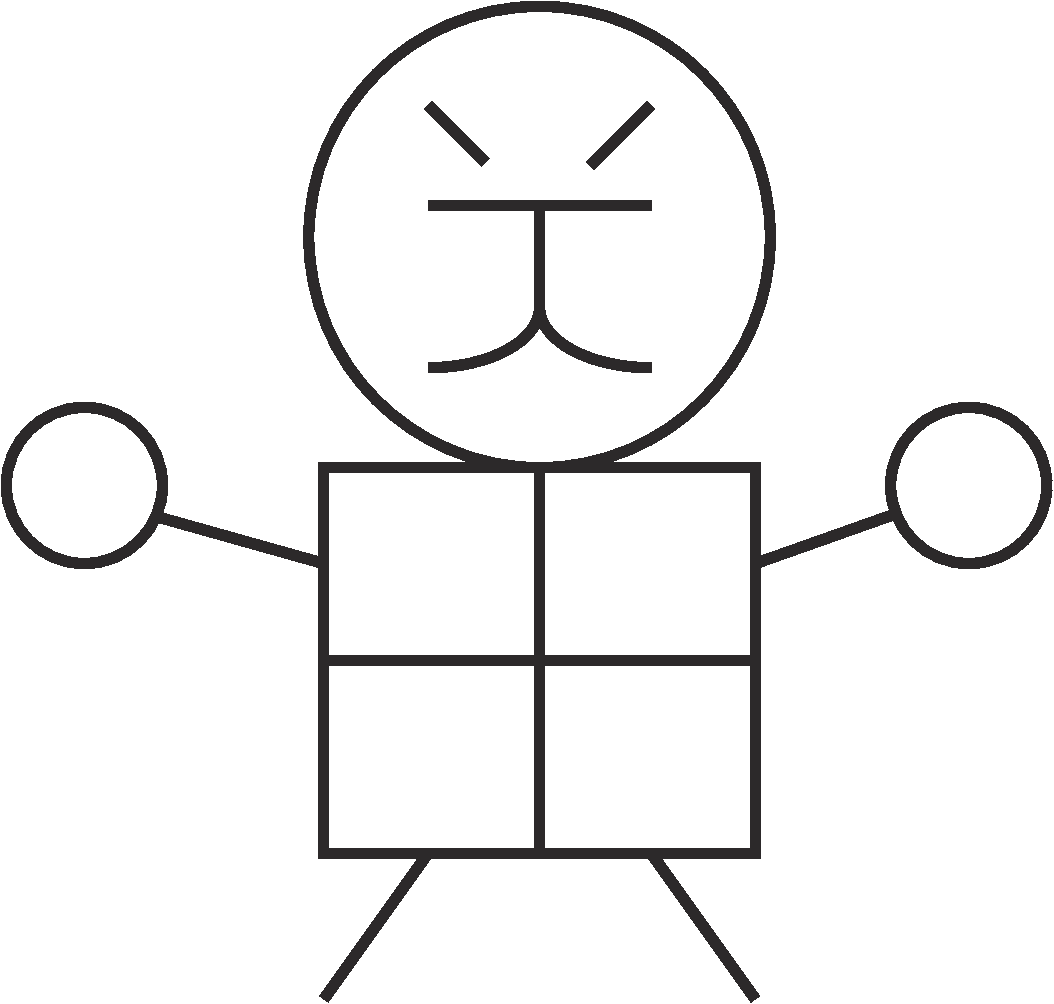
\includegraphics[width=0.3\hsize]{fig/okadakenkun.pdf}  % eps,png,jpg なども可
 \caption{Okadaken-kun. He is a mascot of Okada Lab.}\label{fig:okadakenkun}
\end{figure}
\begin{table}[tbp]
 \centering
 \caption{Young's modulus and Poisson's ratio.}\label{tab:parameters}
 \begin{tabular}{rl}
  \toprule
  Young's modulus (GPa) & 210 \\
  Poisson's ratio & 0.3 \\
  \bottomrule
 \end{tabular}
\end{table}
\section{数式}
数式は
\begin{equation}
 \bm{f} = -k \bm{u}
\end{equation}
のように記します.
複数の数式は
\begin{align}
 \bm{f}_1 = -k \bm{u}_1 \\
 \bm{f}_2 = -k \bm{u}_2
\end{align}
のように記します.
本文中の数式は $\bm{f}$ や $\bm{f} = -k \bm{u}$ のように記します.

label コマンドを付けて
\begin{equation}
 \bm{f} = m \frac{d^2 \bm{u}}{d t^2}\label{eq:motion}
\end{equation}
のように記すと,ref コマンドで式 (\ref{eq:motion}) のように参照できます.
\section{文献の引用}
○○の研究(Okada et al., 1988)のように引用します.
Okada et al.\ (1988) は○○を研究したという書き方の引用もできます.
日本語の場合は,○○の研究(岡田他, 1998)のように引用します.
岡田他(1998)は○○を研究したという書き方の引用もできます.
